% \documentclass[border=0]{standalone}
\documentclass[a3paper]{article}
\usepackage[left=0mm,top=0mm,right=0mm,bottom=0mm]{geometry}
\usepackage{tikz}
% \usetikzlibrary {backgrounds}
\begin{document}
\thispagestyle{empty}
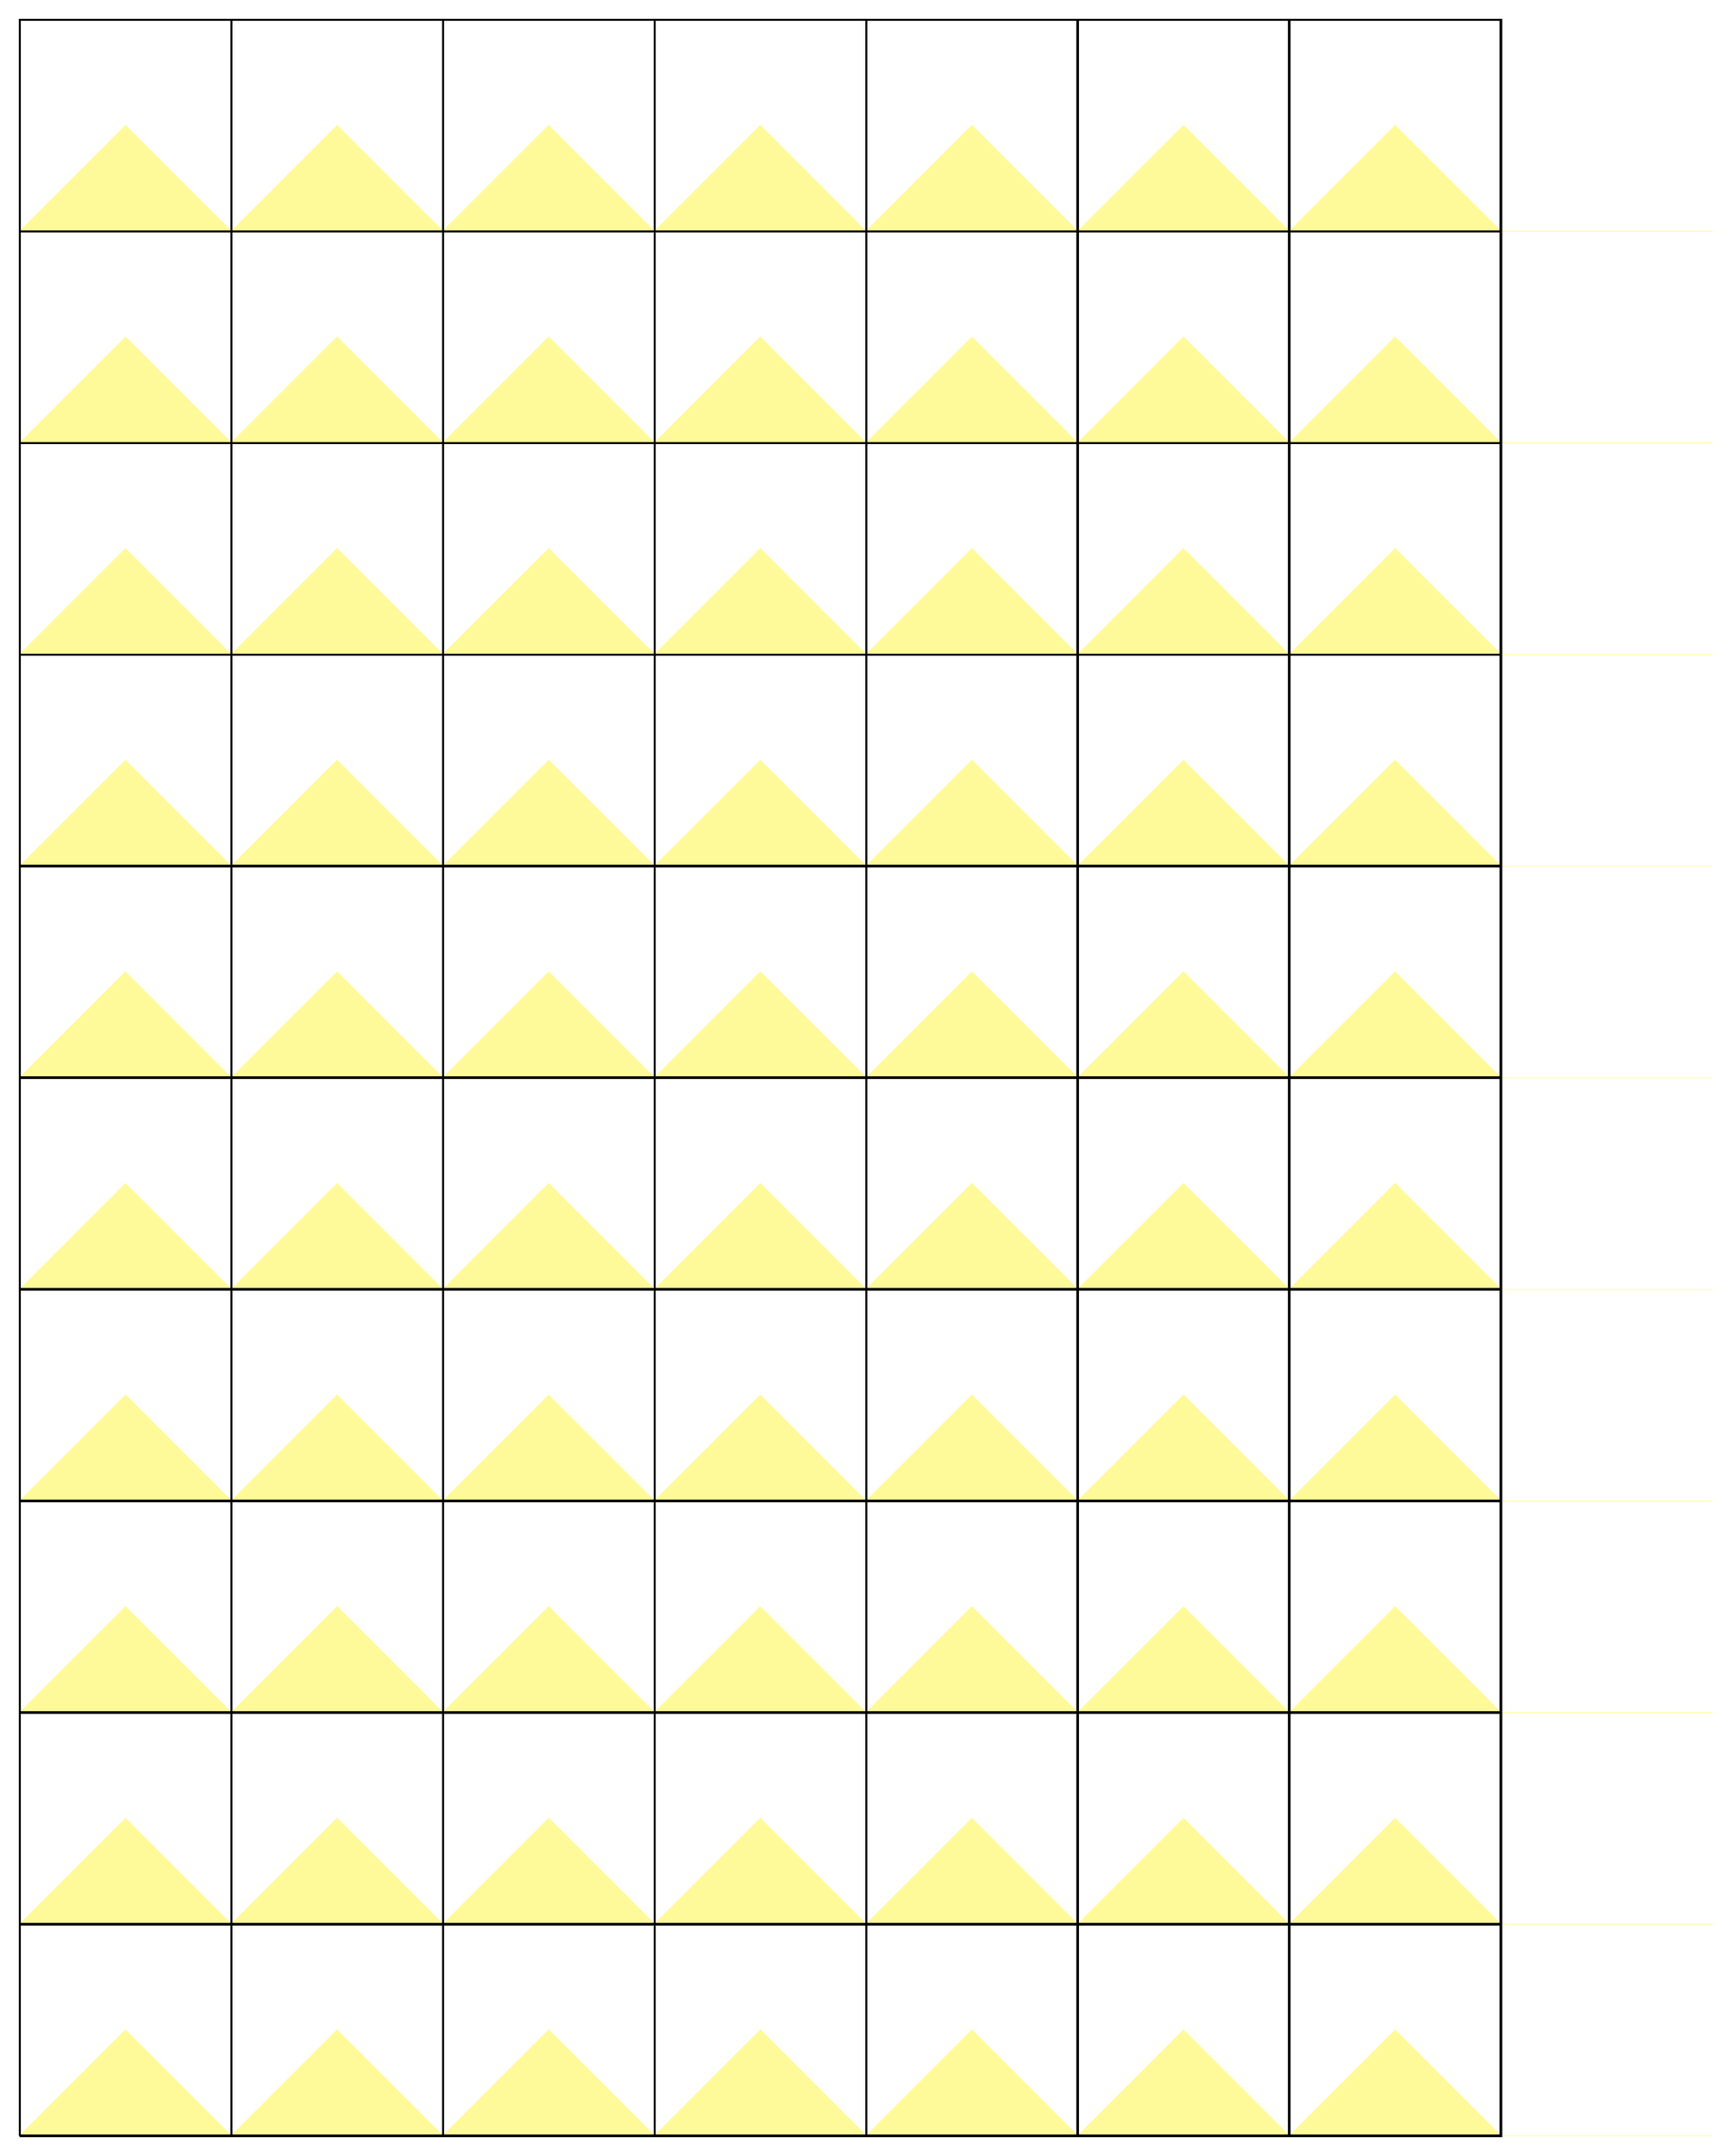
\begin{tikzpicture}
    % \begin{scope}[on background layer={color=cyan!40}]
    %     \fill (-2.5,-.5) rectangle (26,40.5);
    %     \end{scope}
    % \pgfmathsetmacro{\p}{(1+sqrt(5))/2}
    \pgfmathsetmacro{\l}{sqrt(8)}
    \foreach \y in {0,1,2,...,9}{
        \foreach \x in {0,1,...,6}{
            % \filldraw[magenta!40] (4*\x,4*\y) --++ (0:4) --++ (135:\l); 
            \filldraw[yellow!40] (4*\x,4*\y) --++ (45:\l) --++ (315:\l)--++(0:4); 
            \draw[very thick] (4*\x,4*\y) --++ (0:4) --++ (90:4) --++ (180:4) --++ (270:4);
        }
    };

\end{tikzpicture}
\end{document}